\def\duedate{10/27/22}
\def\HWnum{7}
% Document setup
\documentclass[12pt]{article}
\usepackage[margin=1in]{geometry}
\usepackage{fancyhdr}
\usepackage{lastpage}

\pagestyle{fancy}
\lhead{Richard Whitehill}
\chead{MATH 757 -- HW \HWnum}
\rhead{\duedate}
\cfoot{\thepage \hspace{1pt} of \pageref{LastPage}}

% Encoding
\usepackage[utf8]{inputenc}
\usepackage[T1]{fontenc}

% Math/Physics Packages
\usepackage{amsmath}
\usepackage{amssymb}
\usepackage{mathtools}
\usepackage[arrowdel]{physics}
\usepackage{siunitx}

\AtBeginDocument{\RenewCommandCopy\qty\SI}

% Reference Style
\usepackage{hyperref}
\hypersetup{
    colorlinks=true,
    linkcolor=blue,
    filecolor=magenta,
    urlcolor=cyan,
    citecolor=green
}

\newcommand{\eref}[1]{Eq.~(\ref{eq:#1})}
\newcommand{\erefs}[2]{Eqs.~(\ref{eq:#1})--(\ref{eq:#2})}

\newcommand{\fref}[1]{Fig.~\ref{fig:#1}}
\newcommand{\frefs}[2]{Figs.~\ref{fig:#1}--\ref{fig:#2}}

\newcommand{\tref}[1]{Table~\ref{tab:#1}}
\newcommand{\trefs}[2]{Tables~\ref{tab:#1}-\ref{tab:#2}}

% Figures and Tables 
\usepackage{graphicx}
\usepackage{float}

\newcommand{\bef}{\begin{figure}[h!]\begin{center}}
\newcommand{\eef}{\end{center}\end{figure}}

\newcommand{\bet}{\begin{table}[h!]\begin{center}}
\newcommand{\eet}{\end{center}\end{table}}

% tikz
\usepackage{tikz}
\usetikzlibrary{calc}
\usetikzlibrary{decorations.pathmorphing}
\usetikzlibrary{decorations.markings}
\usetikzlibrary{arrows.meta}
\usetikzlibrary{positioning}

% tcolorbox
\usepackage[most]{tcolorbox}
\usepackage{xcolor}
\usepackage{xifthen}
\usepackage{parskip}

\newcommand*{\eqbox}{\tcboxmath[
    enhanced,
    colback=black!10!white,
    colframe=black,
    sharp corners,
    size=fbox,
    boxsep=8pt,
    boxrule=1pt
]}

% Miscellaneous Definitions/Settings
\newcommand{\prob}[2]{\textbf{#1)} #2}
\newcommand{\reals}{\mathbb{R}}
\newcommand{\integers}{\mathbb{Z}}
\newcommand{\naturals}{\mathbb{N}}
\newcommand{\rationals}{\mathbb{Q}}
\newcommand{\complexs}{\mathbb{C}}

\setlength{\parskip}{\baselineskip}
\setlength{\parindent}{0pt}
\setlength{\headheight}{14.49998pt}
\addtolength{\topmargin}{-2.49998pt}







\begin{document}
    
\prob{1}{
Let $A = -\partial^2 : \mathcal{D} \subset L_{2}(-\pi,\pi) \mapsto L_{2}(-\pi,\pi)$, where
$\mathcal{D} = \{ u \in C^2[-\pi,\pi] : u_{x}(-\pi) = u_{x}(\pi) = 0, u(-\pi) = u(\pi) \}$.
Find all eigenvalues and eigenvectors $Ae_{n} = \lambda_{n}e_{n}$.
Hint: Find first the eigenvalues and eigenvectors on $D_{p} = \{ u \in C^2[-\pi,\pi] : u_{x}(-\pi) = u_{x}(\pi), u(-\pi) = u(\pi) \} $ (i.e. periodic boundary conditions).
}

We first solve generally for periodic boundary conditions.
It has been proven in class a few times previously that the eigenvalues of $-\partial^2$ must be positive (using integration by parts).
Let us denote $\lambda = \mu^2$, where $A e(x) = \lambda e(x)$.
It has also been proven that $-\partial^2$ is a hermitian operator, meaning its eigenvalues are all real.
Thus, we have the eigen-equation
\begin{eqnarray}
    \label{eq:eigen-eq}
    \partial_{x}^2e(x) + \mu^2e(x) = 0
.\end{eqnarray}
If $\mu = 0$, then the only eigenfunction admitted is $e(x) = 1$, and if $\mu \ne 0$, then for each $\mu$ we have corresponding eigenfunctions $\cos{\mu x}$ and $\sin{\mu x}$.
In order to satisfy the boundary conditions on $\mathcal{D}_{p}$ we must have that $\mu = n \in \naturals$.

Now, we can extend to the case for our domain $\mathcal{D}$.
Observe that $\partial_{x} \sin{nx} = \cos{n x} = (-1)^{n} \ne 0$, implying that $\sin{nx}$ is not an eigenfunction for $A$.
Thus, our eigenfunctions are $1$ (with corresponding eigenvalue $0$) and $\cos{nx}$ (with corresponding eigenvalues $n^2$ for $n = 1,2\ldots$).
We could combine the two such that our eigenfunctions are $\cos{nx}$ with corresponding eigenvalues $n^2$ for $n = 0,1,\ldots$.

\prob{2}{
Find $u(x,t)$ such that $u_{t} - ku_{xx} = 0$, where $x \in (0,\pi)$, $t>0$, $u(x,0) = \pi^2 - x^2$, $u(0,t) = 0$, and $u(\pi,t) = 0$.
}

We know that the equation $u_{t} - ku_{xx} = 0$ has solution
\begin{eqnarray}
    \label{eq:sol-2}
    \eqbox{
        u(x,t) = e^{-tk\partial_{x}^2} \sum_{n=1}^{\infty} A_{n} \sin{n x} = \sum_{n=1}^{\infty} A_{n} e^{-tkn^2}\sin{nx}
    }
,\end{eqnarray}
where
\begin{eqnarray}
    \label{eq:An}
    \eqbox{
    A_{n} = \frac{2}{\pi}\int_{0}^{\pi} u(x,0) \sin{n x} \dd{x} = \frac{2 \pi^2 n^2 - 4[(-1)^{n} - 1]}{\pi n^3}
}
.\end{eqnarray}



\prob{3}{
Find the Fourier series of $f(x) = \pi^2 - x^2$ on the interval $(-\pi,\pi)$.
Sketch the $2\pi$-periodic extension of $f(x)$.
}

The Fourier series looks as follows (on the interval $[-\pi,\pi]$):
\begin{eqnarray}
    \label{eq:fourier-series}
    f(x) = \frac{a_0}{2} + \sum_{n=1}^{\infty} \big[ a_{n}\cos{n x} + b_{n}\sin{n x} \big]
,\end{eqnarray}
where the coefficients
\begin{align}
    \label{eq:coeffs}
    a_{n} &= \frac{1}{\pi} \int_{-\pi}^{\pi} f(x) \cos{nx} \dd{x} \quad (n=0,1,\ldots) \\
    b_{n} &= \frac{1}{\pi} \int_{-\pi}^{\pi} f(x) \sin{nx} \dd{x} \quad (n=1,2,\ldots)
.\end{align}
Hence, for $f(x) = \pi^2 - x^2$ we have 
\begin{align}
    \label{eq:an}
    a_{n} &= \frac{1}{\pi} \int_{-\pi}^{\pi} (\pi^2 - x^2)\cos{nx} \dd{x} = \frac{2}{\pi} \int_{0}^{\pi} (\pi^2 - x^2) \cos{nx} \dd{x} \\
          &= -\frac{4\cos{n\pi}}{n^2} = -\frac{4(-1)^{n}}{n^2}
,\end{align}
and $b_{n} = 0$ since $f(x)$ is even. 
Thus,
\begin{eqnarray}
    \label{eq:fourier-pix}
    \eqbox{
    \pi^2 - x^2 = \frac{2\pi^2}{3} -4\sum_{n=1}^{\infty} \frac{(-1)^{n}}{n^2}\cos{nx}
}
.\end{eqnarray}

We could also have found this result from the result of problem 5:
\begin{align}
    \label{eq:3-from-5}
    \frac{3x^2 - \pi^2}{12} = -\frac{(\pi^2 - x^2)}{4} +\frac{\pi^2}{6} &= \sum_{n=1}^{\infty} \frac{(-1)^{n}}{n^2}\cos{nx} \\
    \Rightarrow \pi^2 - x^2 &= \frac{2\pi^2}{3} - 4\sum_{n=1}^{\infty} \frac{(-1)^{n}}{n^2} \cos{nx}
,\end{align}
which is the result we found above in \eref{fourier-pix}.

Additionally, we can sketch the $2\pi$-periodic continuation of $f(x)$ as below.
Note that this is only a sketch.
These are meant to be parabolas (not half circles).
\begin{center}
    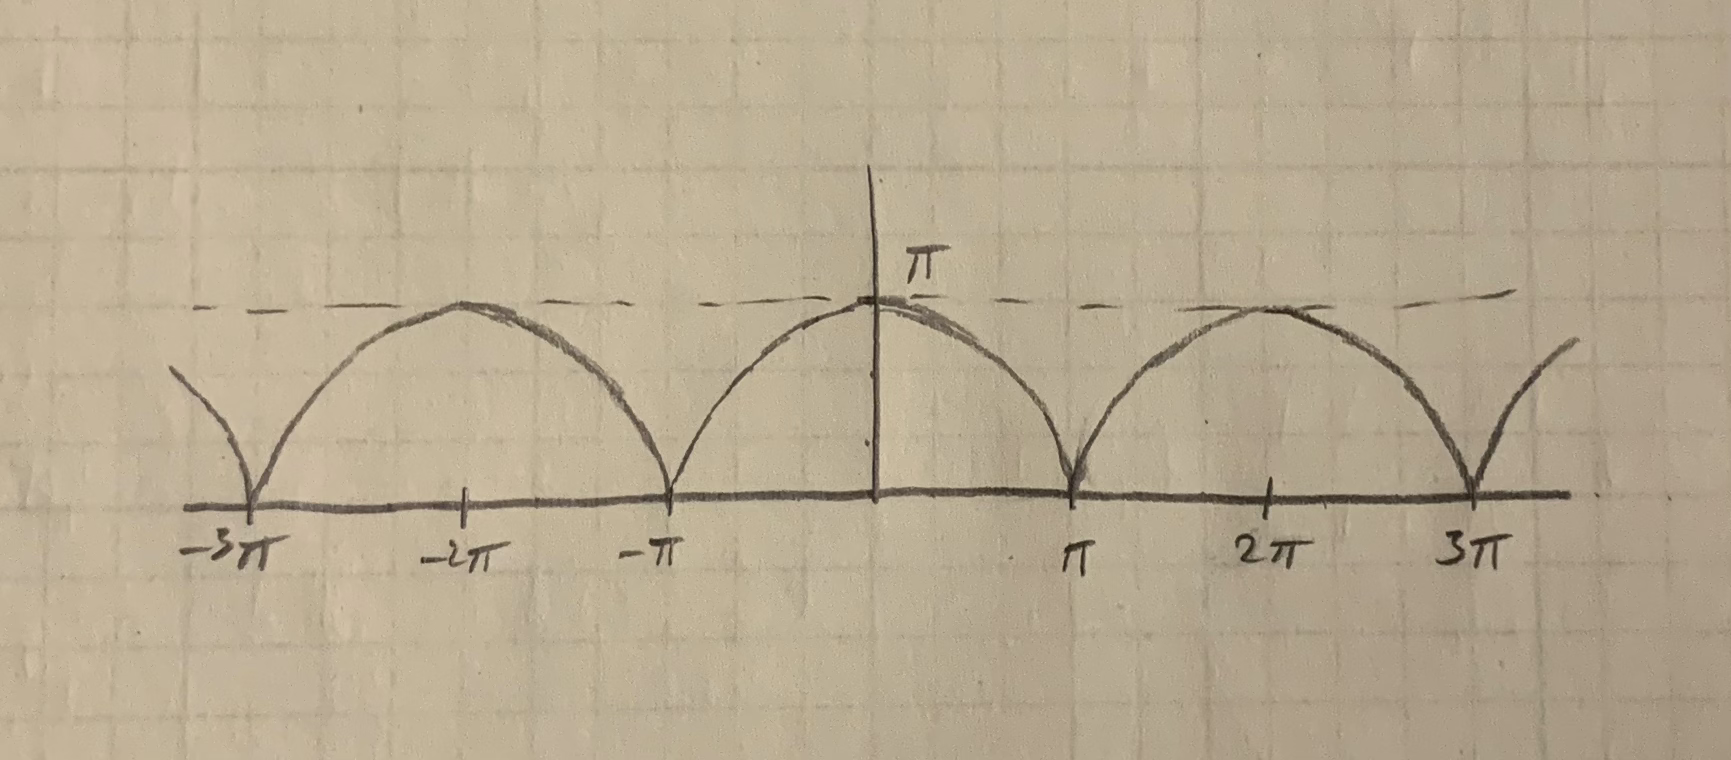
\includegraphics[width=0.8\textwidth]{prob3.png}
\end{center}


\prob{4}{
Check the identity
\begin{eqnarray}
    \label{eq:id-4}
    \sum_{n=1}^{\infty} \frac{1}{n^2} \cos{nx} = \frac{1}{12}\big( 3x^2 - 6 \pi x + 2\pi^2 \big)
,\end{eqnarray}
where $0 \leq x \leq 2\pi$.
}

Observe that $\sin^2{(nx/2)} = (1 - \cos{nx})/2$ for any $x$.
Thus, 
\begin{eqnarray}
    \label{eq:sum-rewrite}
    \sum_{n=1}^{\infty} \frac{1}{n^2}\cos{(nx)} = \sum_{n=1}^{\infty} \frac{1}{n^2} (1 - 2\sin^2{(nx/2)}) = \frac{\pi^2}{6} - 2\sum_{n=1}^{\infty} \frac{1}{n^2} \sin^2{(nx/2)} 
.\end{eqnarray}
Notice that
\begin{eqnarray}
    \label{eq:2sin}
    2\sum_{n=1}^{\infty} \frac{\sin^2{(nx/2)}}{n^2} = \sum_{n=-\infty}^{\infty} \frac{\sin^2{(nx/2)}}{n^2} - \Big( \frac{x}{2} \Big)^2
,\end{eqnarray}
where the $n=0$ term is the limiting value of $(\sin{(nx/2)}/n)^2$ as $n \rightarrow 0$, which is just $(x/2)^2$.
Hence,
\begin{align}
    \label{eq:sum-rewrite-2}
    \eqbox{
        \begin{aligned}
    \sum_{n=1}^{\infty} \frac{\cos{(nx)}}{n^2} &= \frac{\pi^2}{6} + \frac{x^2}{4} - \sum_{n=-\infty}^{\infty} \frac{\sin^2{(nx/2)}}{n^2} = \frac{\pi^2}{6} + \frac{x^2}{4} - \frac{\pi x}{2} \\
                                               &= \frac{1}{12}\big( 3x^2 - 6 \pi x + 2\pi^2 \big)
        \end{aligned}
                                           }
,\end{align}
where we have used the result that 
\begin{eqnarray}
    \label{eq:result-used}
    \pi u = \sum_{n=-\infty}^{\infty} \frac{\sin^2{(nu)}}{n^2}
,\end{eqnarray}
on the interval $u \in (0,\pi)$.

This is proven using Parseval's theorem with the function $\displaystyle f(x) = \begin{cases} \pi & |x| < u \\ 0 & |x| > u \end{cases}$.
Then, on the interval $(-u,u)$ we have
\begin{eqnarray}
    \label{eq:f-fourier}
    f(x) = \sum_{n=-\infty}^{\infty} c_{n} e^{inx}
,\end{eqnarray}
where
\begin{eqnarray}
    \label{eq:cn}
    c_{n} = \frac{1}{2\pi}\int_{-u}^{u} \pi e^{inx} \dd{x} = \frac{\sin{nu}}{n}
.\end{eqnarray}
Parseval's theorem then states that
\begin{eqnarray}
    \label{eq:parseval}
    \sum_{n=-\infty}^{\infty} |c_{n}|^2 = \sum_{n=-\infty}^{\infty} \frac{\sin^2(nu)}{n^2} = \frac{1}{2\pi}\int_{-u}^{u} |f(x)|^2 \dd{x} = \pi u
.\end{eqnarray}







\prob{5}{
Check the identity
\begin{eqnarray}
    \label{eq:id-5}
    \sum_{n=1}^{\infty} \frac{(-1)^{n}}{n^2} \cos{nx} = \frac{1}{12}(3x^2 - \pi^2)
,\end{eqnarray}
where $x \in [-\pi,\pi]$.
}

The fourier series for $f(x) = (3x^2 - \pi^2)/12$ is given by
\begin{eqnarray}
    \label{eq:fourier-series-5}
    \frac{3x^2 - \pi^2}{12} = \frac{a_0}{2} + \sum_{n=1} a_{n}\cos{nx} 
,\end{eqnarray}
where the sine terms vanish since $f(x)$ is an even function and
\begin{align}
    \label{eq:an-coeffs-5}
    a_{0} &= \frac{1}{6\pi} \int_{0}^{\pi} (3x^2 - \pi^2) \dd{x} = 0 \\
    a_{n>0} &= \frac{1}{6\pi} \int_{0}^{\pi} (3x^2 - \pi^2) \cos{nx} \dd{x} = \frac{(-1)^{n}}{n^2}
.\end{align}
Hence,
\begin{eqnarray}
    \label{eq:result-5}
    \eqbox{
    \frac{1}{12}(3x^2 - \pi^2) = \sum_{n=1}^{\infty} \frac{(-1)^{n}}{n^2} \cos{nx}
}
.\end{eqnarray}


\prob{6}{
Find $\displaystyle \sum_{n=1}^{\infty} \frac{1}{n^2}$ using the result of problem 4 or 5.
}

Using $x = 0$ with \eref{id-4}, we find
\begin{eqnarray}
    \label{eq:id-6}
    \eqbox{
    \sum_{n=1}^{\infty} \frac{1}{n^2} = \frac{2\pi^2}{12} = \frac{\pi^2}{6} 
}
.\end{eqnarray}


\prob{7}{
Find $\displaystyle \sum_{n=1}^{\infty} \frac{(-1)^{n}}{n^2}$ using the result of problem 5 or 4.
}

Using $x = 0$ with \eref{id-5}, we find
\begin{eqnarray}
    \label{eq:id-7}
    \eqbox{
    \sum_{n=1}^{\infty} \frac{(-1)^{n}}{n^2} = -\frac{\pi^2}{12}
}
.\end{eqnarray}



\end{document}
